%
% am.tex -- Amplitudenmodulation
%
% (c) 2018 Prof Dr Andreas Müller, Hochschule Rapperswil
%
\documentclass[tikz,12pt]{standalone}
\usepackage{times}
\usepackage{amsmath}
\usepackage{txfonts}
\usepackage[utf8]{inputenc}
\usepackage{graphics}
\usepackage{color}
\usepackage{pifont}
\usetikzlibrary{arrows,intersections,math,calc}
\begin{document}

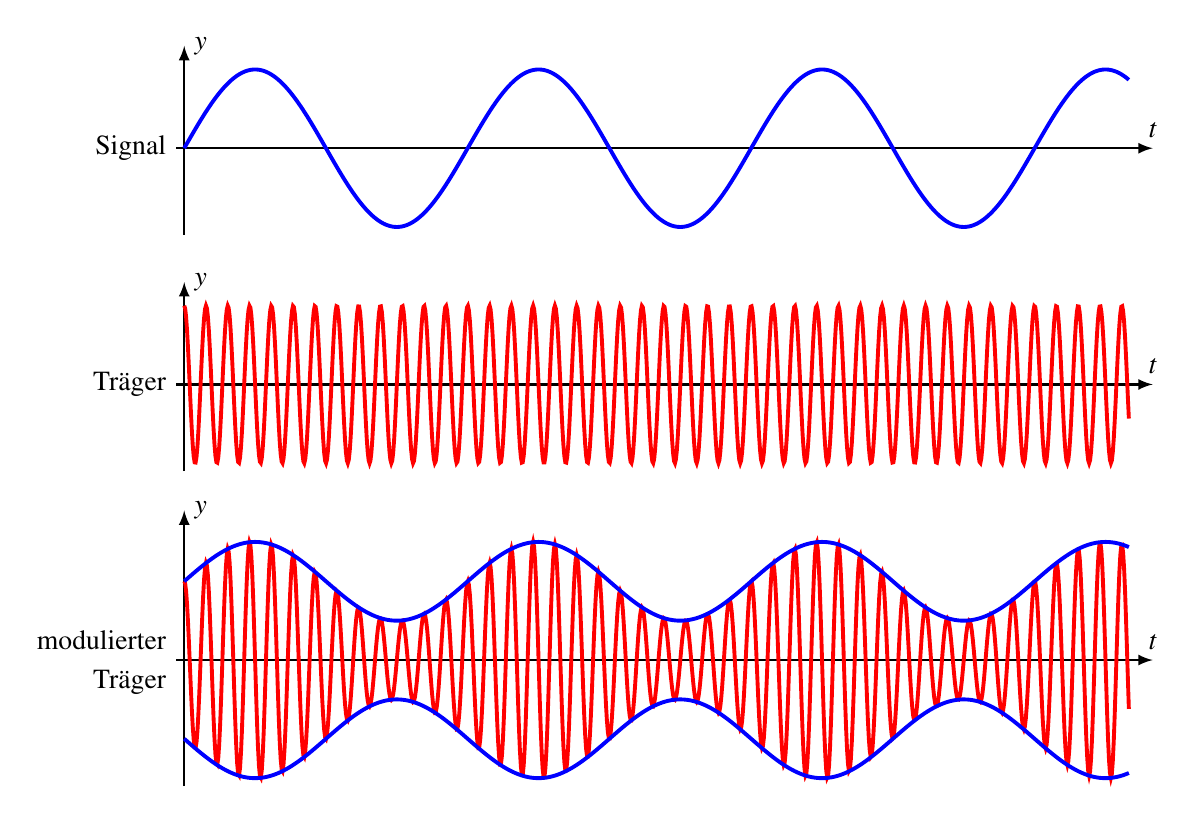
\begin{tikzpicture}[>=latex,thick]

\def\s{1300}

\begin{scope}[yshift=3cm]
\draw[->] (-0.1,0)--(12.3,0) coordinate[label={$t$}];
\draw[->] (0,-1.1)--(0,1.3) coordinate[label={right:$y$}];

\draw[color=blue,line width=1.4pt] plot[domain=0:12,samples=1000]
	({\x},{sin(100*\x)});
\node at (-0.1,0) [left] {Signal};
\end{scope}

\begin{scope}
\draw[->] (-0.1,0)--(12.3,0) coordinate[label={$t$}];
\draw[->] (0,-1.1)--(0,1.3) coordinate[label={right:$y$}];

\draw[color=red,line width=1.4pt] plot[domain=0:12,samples=1000]
	({\x},{cos(\s*\x)});
\node at (-0.1,0) [left] {Träger};
\end{scope}

\begin{scope}[yshift=-3.5cm]
\draw[->] (-0.1,0)--(12.3,0) coordinate[label={$t$}];
\draw[->] (0,-1.6)--(0,1.9) coordinate[label={right:$y$}];

\draw[color=red,line width=1.4pt] plot[domain=0:12,samples=1000]
	({\x},{(1+0.5*sin(100*\x))*cos(\s*\x)});
\draw[color=blue,line width=1.4pt] plot[domain=0:12,samples=1000]
	({\x},{1+0.5*sin(100*\x)});
\draw[color=blue,line width=1.4pt] plot[domain=0:12,samples=1000]
	({\x},{-1-0.5*sin(100*\x)});

\node at (-0.1,0) [above left] {modulierter};
\node at (-0.1,0) [below left] {Träger};
\end{scope}

\end{tikzpicture}

\end{document}

